\chapter{提案手法}
\label{proposal}
\section{本提案手法の位置付け}
\label{issue-to-solve}
本章では,\ref{sensing-by-vanet}項にて述べた駐車区画の満空情報を共有する手法群や利用車両のナビゲーションを行う手法群を運用する際に,前提条件となる駐車区画の位置関係や収容台数を表すネットワークモデルの自律的な推定手法について述べる.

本研究では,車両の位置情報や駐車情報の収集に際しては\ref{ivi}節で述べたような車載アプリケーションプラットフォームによって行うと想定する.これによりVANETのような専用機器を用いる手法と比較して普及の容易度を高めることが出来る.

\ref{gps-gen-map}項で述べたように,KDE法を中心とした様々なアルゴリズムを用いることで,位置情報ログデータから道路地図は安定して生成出来ることが明らかにされている.しかしながら,駐車場のネットワークモデルを構築するためには駐車区画の位置情報,駐車枠数のパラメーターが必要になる.本研究ではこれらのパラメーターの推定手法に関して検討する.


\section{用語}
本論文内で用いる用語について,以下に定義する.
また,図\ref{networkmodel-example}に本論文で定義する用語とネットワークモデルの概念図を示す.
\begin{figure}
	\centering
	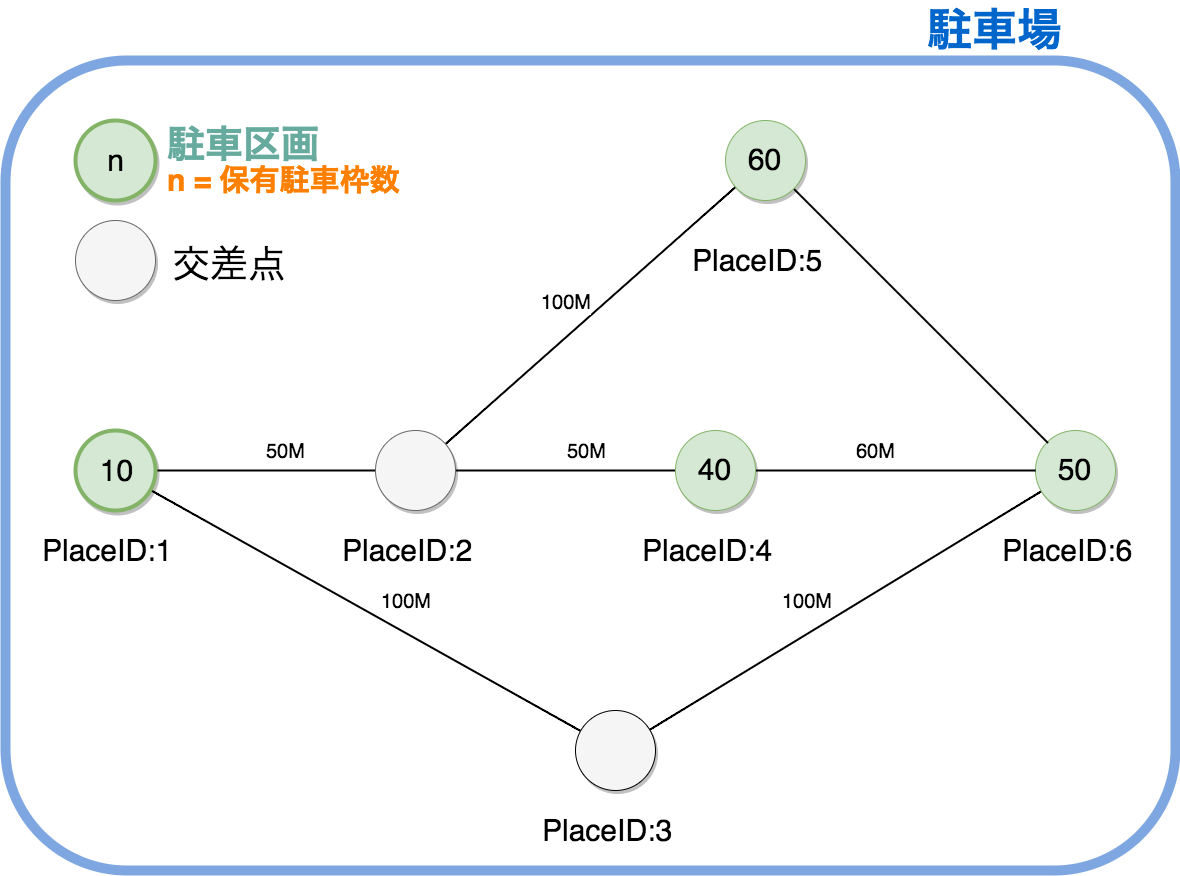
\includegraphics[width=10cm]{fig/networkmodel.png}
	\caption{本研究で定義するネットワークモデルの例}
	\label{networkmodel-example}
\end{figure}
\begin{itemize}
	\item 駐車区画:車両が駐車可能な枠が隣接する場所を指す.一つの駐車区画は駐車枠を単数あるいは複数持つ.
	% parking block
	\item 駐車場:駐車区画群を持つ施設全体を示す.
	% paking area
	\item 駐車枠:車両一台を駐車出来る箇所を指す.本論文,提案手法では車両の大きさによる駐車枠の違いは考慮しない.
	% pakrking lot
	\item ネットワークモデル:座標$\cdot$駐車枠の数をパラメーターに含む駐車場内の駐車区画を表すノードと,それらを結ぶ道路を表す重み付きエッジを含むデータ構造と定義する.ネットワークグラフの形で視覚的に表現することが出来る.
	\item 交差点:複数の道路が接続されている地点を差す.駐車場をネットワークモデルとして表した場合,駐車枠を持たないノードが交差点にあたる.
\end{itemize}


\section{目的と仮説}
\label{purpose-proposal}
\subsection{本提案手法の目的}
本提案手法では既存の駐車場内効率化手法$\cdot$ネットワークモデル構築手法の諸問題に以下のように取り組む.

\subsubsection{運営主体に依存しないアーキテクチャ}
\ref{issue-to-solve}節でも述べたように,駐車場内に常設されたセンサーにより満空情報を管理する従来のアーキテクチャでは,運営主体が負担できるコストに実施性を依存していた.そのため余分な運用コストを費やすことの出来ない駐車場施設では,利用者の利便性の向上が困難であった.

また,\ref{sensing-by-vanet}項で指摘したように,車両側のセンサーを活用する手法では,ネットワークモデルの事前構築が必要という点で,結果的に運営主体による維持$\cdot$管理が必要であった.

本提案手法では,運営主体に依らない駐車場効率化手法を実現可能にするためのネットワークモデルの自律的な推定を目指す.
\subsubsection{駐車場を含めたネットワークモデルの構築}
\ref{gps-gen-map}節で述べた道路地図推定手法では,駐車場の推定には焦点が当てられていなかった.
本研究では駐車場の位置推定を可能にするアーキテクチャを提案する.

\subsubsection{敷設センサーやRSUが不要}
第\ref{related}章でも述べたように,既存の多くの駐車場最適化手法では路上側にセンサーや通信機器(RSU)を設置する必要があった.利用車両の位置情報測位システムと携帯電話回線網を用いる本提案手法では,路側に常設する機器が必ずしも必要にならない.そのため,駐車場の運営者による投資が難しい非営利施設の駐車場でも,駐車場効率化サービスを運用することが可能になる. 

%以下はまとめにFutureworkに引っ越しする予定
%\subsubsection{複数の駐車場の統合的な管理の実現}
%本論文では単一駐車場内のネットワークモデルを推定することに焦点を当てているが,本提案手法を応用することによって,複数の駐車場を含めたネットワークモデル推定へと対象の範囲を拡げる事も可能になる.
%以下はまとめにFutureworkに引っ越しする予定
%\subsubsection{変更追従性}
%\ref{sensing-by-vanet}節で述べた既存の手法群では通行止めや駐車区画配置の変更によって新たにネットワークモデルを再設定する必要があった.本手法では利用車両の実際の使用ログを収集するため,ネッ%トワークモデルの変更にある程度の追従性を持たせる設計を行うことが可能になる.


\subsection{本研究の仮説}
本研究では,\ref{issue-to-solve}節で述べたような既存の駐車場効率化手法の諸問題の解決に取り組む.
自動車の位置情報を収集$\cdot$解析することで,駐車区画の設定や最大収容台数を駐車場ごとに設定したり路側にセンサーを常設することなく、駐車区画の空き状況を収集$\cdot$可視化することが出来るようになると予想している.

\section{本提案手法の仮定と設計}
\subsection{位置情報の収集と提供}
本提案手法には駐車場を利用する車両の位置情報を収集する機構が必要になる.ここでは位置情報収集システムに関して述べる.

\subsubsection{車載器とサービスクライアント}
\ref{ivi}節で述べたような自動車用アプリケーションプラットフォーム上で動作するサービスクライアントを利用者の車両で動作させる.サービスクライアントは携帯電話回線網を用いて,自動車の位置情報をサービスサーバーに定期的に送信する.また,車両が駐車した場合にエンジンの停止を検知して駐車シグナルを同時に送信するものとする.

\subsubsection{サービスサーバー}
本提案手法では,情報を収集しネットワークモデルを推定するサービスサーバーの実装を想定する.サービスクライアントとサービスサーバ間はインターネットを介して接続される.

\subsubsection{ネットワークモデルを利用するアプリケーション}
満空情報の可視化や駐車場内のナビゲーションを行う様々なアプリケーションを運営するサーバーをアプリケーションサーバーと定義する.サードパーティによるアプリケーションのリリースを想定し,アプリケーションサーバーは,サービスサーバーとは別に構築する.アプリケーションサーバーはサービスサーバーからネットワークモデルや車両の位置情報の提供を受ける.

アプリケーションのクライアントは必ずしも車載された端末である必要はなく,WEBサービスやスマートフォン上で動作するアプリケーションを介して利用者にサービスを提供する形を想定する.


\begin{figure}
	\centering
	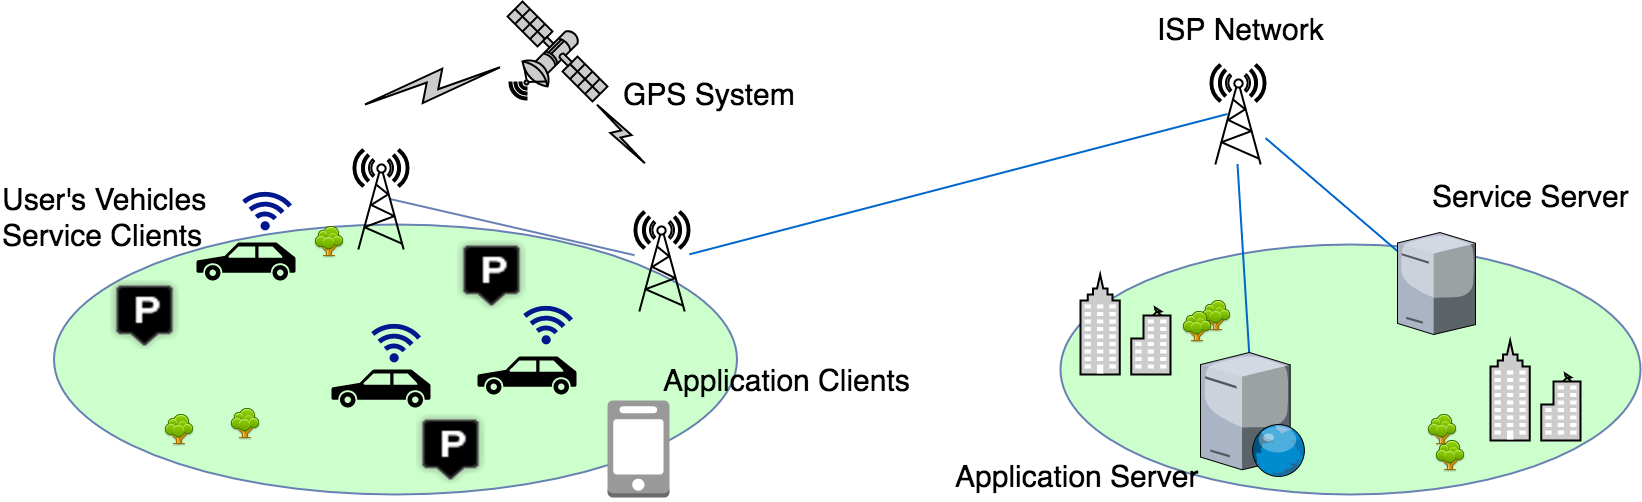
\includegraphics[width=15cm]{fig/network-concept.png}
	\caption{本提案手法での各ホストのコンセプト}
	\label{network-concept}
\end{figure}


\subsection{駐車区画の位置推定}
\label{how-to-park-area}
一定期間において収集された利用車両の駐車シグナルを受けた座標群から,X-Means法を用いてクラスタリングを行い,各クラスターの重心値を駐車区画の位置座標と推定する.

\subsubsection{X-Means法}
X-Means法とはPellegらによって提案された非階層型クラスタリングアルゴリズムである\cite{Pelleg}.
クラスタ数の決定を行うために発見的方法に頼る必要があったk-Means法の発展形として考案された手法で,クラスター数をデータセットに合わせて推定し,データ群を適切な数のクラスターに分けることが出来る.


X-Means法の基本的なアルゴリズムを下記に簡便に表す.
\begin{enumerate}
	\item $n$個の$p$次元行列のデータセットを用意する.
	\item 始めに$k=2$としてk-Means法を実行し2つのクラスターにデータを分割する.
	\item 各クラスタをベイズ情報量基準(BIC)などの情報量基準尺度を用いて評価し,2クラスタに分けることが適当と判断できる場合,そのクラスタ内で2.を実行する.そうでない場合にそのクラスタの分割を終了する.
	\item 全てのクラスタの分割が終了するまで2.と3.を継続する.
\end{enumerate}

本提案手法では,Pelleg手法を一部改良した石岡手法\cite{Ishioka}を採用した.石岡手法ではクラスタリングしたデータ群が必ずしもガウス分布していないことを考慮しているため,多様なパターンのデータへの汎用性が高い.





\subsection{駐車区画の駐車枠数の推定}
\label{how-to-park-slot}
\ref{how-to-park-area}項で推定された駐車区画の座標を基に,駐車ログ群がどの駐車区画で行われたものかを推定し,
同一単位時間中$t$の最大駐車台数をその駐車区画の保有駐車枠数とする.
駐車区画の枠数$S_p$は以下のような数式で表される.
\begin{align}
	S_p = \max \{ f(t),t = 1,2 \cdots,\max\{t\} \}       \\
	S_p \leq G_p										\\
	G_p = pの保有する駐車枠数の真値\\
	f(t) = 単位時間t時のpに駐車している車両台数                   \\
	t = 単位時間                                     \\
	\max\{t\} = 推定対象とするデータセットの時間 
\end{align}

\subsection{道路地図の推定}
道路地図の生成には,走行ログデータ(駐車時以外の位置情報ログデータ群)を用いる.

走行ログデータから,\ref{gps-gen-map}節にて述べたDaviesらによる手法\cite{Davies}などを用いて道路地図を推定する.

生成された道路地図上に\ref{how-to-park-area}節で求められた駐車区画を割り当てる.


\section{フロー図}
\begin{figure}
	\centering
	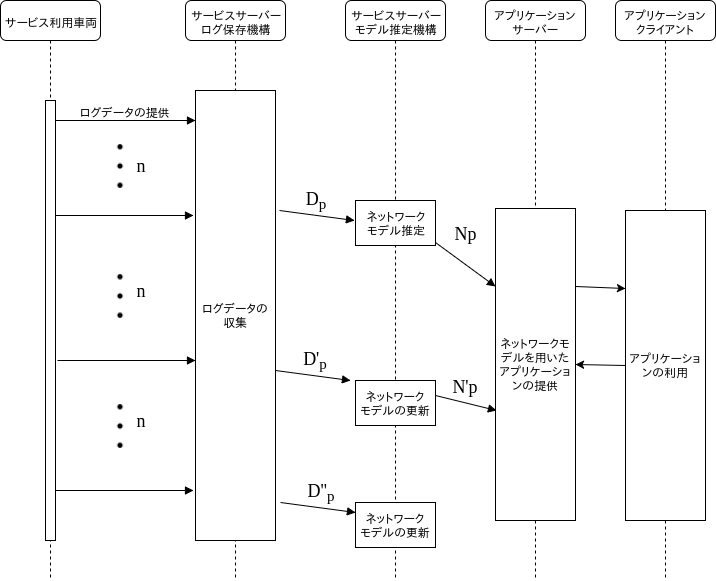
\includegraphics[width=14cm]{fig/flow_proposal.png}
	\caption{本提案手法のフローチャート}
	\label{flow_proposal}
\end{figure}
図\ref{flow_proposal}に本提案手法のフローを表す.以下に具体的な動作を列挙する.
\begin{enumerate}
	\item データの収集\\
	      利用車両の車載端末から位置情報を収集する.推定対象とするデータセットの時間$n$の間に,駐車場$P$に進入した車両から収集したネットワークモデル推定に用いるデータセットを$D_p$とする.
	\item ネットワークモデルの推定\\
	      データセット$D_p$に対して第\ref{how-to-park-area}項にて述べた手法で解析を行う.その結果を推定されたネットワークモデル$N_p$とする.
	\item ネットワークモデルの提供\\
	      ネットワークモデルを利用するアプリケーションに$N_p$を提供する.
	      以降,$n$が経過するたびに1.と2.を繰り返し,あらたに得られたデータセット$D'_p$から推定した結果$N'_p$を駐車場$P$のネットワークモデルとする.
	\item アプリケーションの提供\\
	      サービスサーバーに蓄積された各駐車場のネットワークモデルを,様々なアプリケーションが使用することを想定する.図\ref{flow_proposal}では駐車場$P$のネットワークモデルをアプリケーションサーバーが利用する. アプリケーションサーバーはアプリケーションクライアントと相互に通信し,満空状況の可視化のような駐車場の効率化サービスを提供する.
\end{enumerate}
